\documentclass{standalone}
\usepackage[utf8]{inputenc}
\usepackage{amsmath}
\usepackage{amsfonts}
\usepackage{amssymb}
\usepackage{xparse}
\usepackage{physics}
\usepackage{tikz}
\usetikzlibrary{intersections}
\author{Disha J. Kuzhively}
\begin{document}
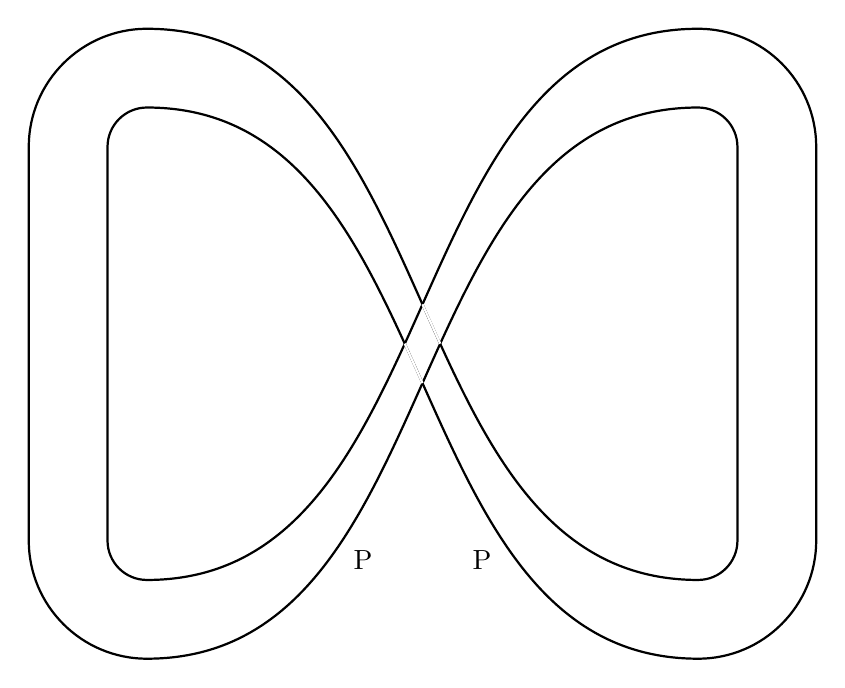
\begin{tikzpicture}
% \draw (0,0) grid (7,5);
\coordinate (A) at (1.5,-1.5);
\coordinate (B) at (1.5,-0.5);
\coordinate (C) at (8.5,-1.5);
\coordinate (D) at (8.5,-0.5);
\draw[thick, name path=curveA] (A) arc [start angle=270, end angle=180, radius=1.5] --+ (90:5) arc [start angle=180, end angle=90, radius=1.5] to[out=0, in=180] (D);
\draw[thick, name path=curveB] (B) arc [start angle=270, end angle=180, radius=0.5] --+ (90:5) arc [start angle=180, end angle=90, radius=0.5] to[out=0,in=180] (C);
\draw[thick, name path=curveC] (C) arc [start angle=270, end angle=360, radius=1.5] --+ (90:5) arc [start angle=0, end angle=90, radius=1.5] to[out=180,in=0] (B);
\draw[thick, name path=curveD] (D) arc [start angle=270, end angle=360, radius=0.5] --+ (90:5) arc [start angle=0, end angle=90, radius=0.5] to[out=180,in=0] (A);
\draw[name intersections={of=curveA and curveD}] (intersection-3)[white,thick] -- (5,3);
\draw[name intersections={of=curveB and curveC}] (intersection-3)[white,thick] -- (5,2);
\draw (4,0) node[below right] {P};
\draw (6,0) node[below left] {P};
\end{tikzpicture}
\end{document}